\PassOptionsToPackage{table}{xcolor}
\documentclass[12pt,letterpaper,twocolumn,openany,nodeprecatedcode,bg=none]{dndbook}
\usepackage[english]{babel}
\usepackage[utf8]{inputenc}
\usepackage{longtable,booktabs,array}
\usepackage{calc}
\usepackage{etoolbox}
\usepackage{caption}
\usepackage{float}
\usepackage{graphicx}
\usepackage{needspace}
\usepackage{tikz}

% Reset zebra striping at the start of every table
\AtBeginEnvironment{longtable}{\rowcolors{1}{white}{gray!10}\small}
\AtBeginEnvironment{table}{\rowcolors{1}{white}{gray!10}}

\providecommand{\pandocbounded}[1]{#1}
\providecommand{\tightlist}{%
  \setlength{\itemsep}{0pt}\setlength{\parskip}{0pt}}

\captionsetup{labelformat=empty}
\setcounter{secnumdepth}{0}
\setlength{\parindent}{0pt}
\setlength{\parskip}{0.5\baselineskip}
\setlength{\headheight}{15pt}

% Prevent orphaned subsections
\let\oldsubsection\subsection
\renewcommand{\subsection}[1]{%
  \needspace{5\baselineskip}%
  \oldsubsection{#1}%
}

\begin{document}
\onecolumn

      \title{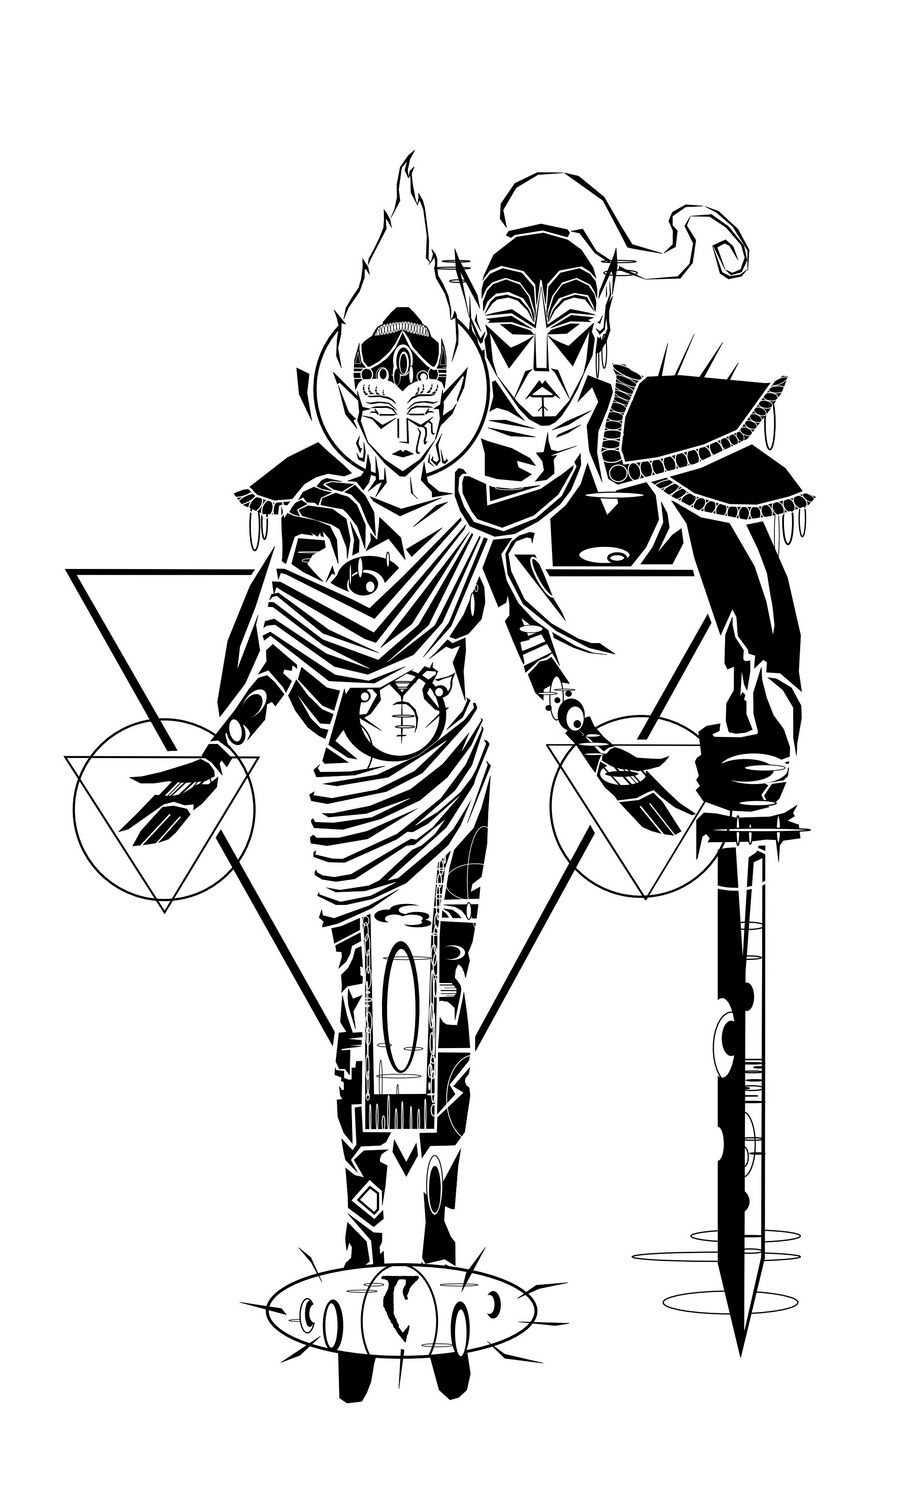
\includegraphics[width=0.9\textwidth,height=0.55\textheight,keepaspectratio]{almalexia.jpg}\\[1.5cm]Mystic
of Lore}
  \author{Class Handbook}
\date{}
\maketitle


\clearpage
\thispagestyle{empty}
\begin{center}
\vspace*{\fill}
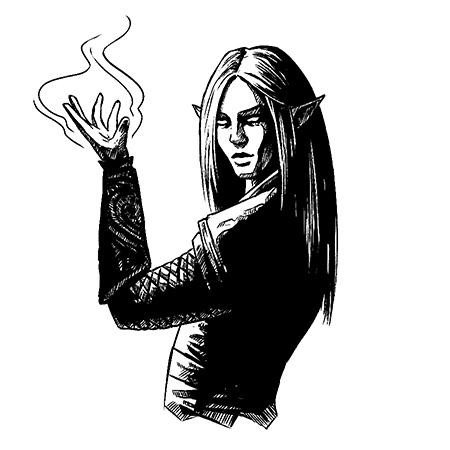
\includegraphics[width=\textwidth,height=0.85\textheight,keepaspectratio]{elfMage.jpg}\par
\vspace{0.4cm}
{\itshape There are many mysteries in the arcane arts.}\par
\vspace*{\fill}
\end{center}

\clearpage
\twocolumn

\section{Mystic (Lore)}\label{mystic-lore}

\subsection{Core Mystic (Lore) Traits}\label{core-mystic-lore-traits}

\needspace{11\baselineskip}

{\def\LTcaptype{none} % do not increment counter
\begin{table}[!htbp]
\centering
\begin{tabular}{@{}
  >{\raggedright\arraybackslash}p{(\linewidth - 2\tabcolsep) * \real{0.3939}}
  >{\raggedright\arraybackslash}p{(\linewidth - 2\tabcolsep) * \real{0.6061}}@{}}
\toprule\noalign{}
\begin{minipage}[b]{\linewidth}\raggedright
\textbf{Primary Ability}
\end{minipage} & \begin{minipage}[b]{\linewidth}\raggedright
Intelligence
\end{minipage} \\
\midrule\noalign{}
\textbf{Hit Points} & 1d4 \\
\textbf{Saving Throw Proficiencies} & Intelligence, Wisdom \\
\textbf{Skill Proficiencies} & Choose 2 skills \\
\textbf{Weapon Proficiencies} & Choose 1 category \\
\textbf{Starting Equipment} & Breastplate, 2 Daggers, Staff, Orb,
Robe \\
\bottomrule\noalign{}
\end{tabular}
\end{table}
}

\subsection{Mystic (Lore) Features}\label{mystic-lore-features}

\needspace{20\baselineskip}

{\def\LTcaptype{none} % do not increment counter
\begin{table}[!htbp]
\centering
\begin{tabular}{@{}
  >{\raggedright\arraybackslash}p{(\linewidth - 4\tabcolsep) * \real{0.1087}}
  >{\raggedright\arraybackslash}p{(\linewidth - 4\tabcolsep) * \real{0.2391}}
  >{\raggedright\arraybackslash}p{(\linewidth - 4\tabcolsep) * \real{0.6522}}@{}}
\toprule\noalign{}
\begin{minipage}[b]{\linewidth}\raggedright
Level
\end{minipage} & \begin{minipage}[b]{\linewidth}\raggedright
Proficiency
\end{minipage} & \begin{minipage}[b]{\linewidth}\raggedright
Class Features
\end{minipage} \\
\midrule\noalign{}
1 & +2 & Spellcasting, Mystic Knowledge \\
2 & +2 & --- \\
3 & +2 & Ability Bonus \\
4 & +2 & --- \\
5 & +2 & Wise and Studied \\
6 & +2 & --- \\
7 & +2 & Ability Bonus \\
8 & +2 & --- \\
9 & +3 & --- \\
10 & +3 & --- \\
\bottomrule\noalign{}
\end{tabular}
\end{table}
}

\subsection{Level 1: Spellcasting}\label{level-1-spellcasting}

You can cast spells from the Mystic (Lore) spell list. Intelligence is
your casting ability. You know two cantrips.

You prepare a number of spells equal to your total number of spell
slots. You may change your prepared spells after an extended period of
downtime.

You regain all expended spell slots when you finish a long rest. Once
per day, you may regain 1 expended spell slot when you finish a short
rest.

\subsection{Spell Slots by Level}\label{spell-slots-by-level}

\needspace{20\baselineskip}

{\def\LTcaptype{none} % do not increment counter
\begin{table}[!htbp]
\centering
\begin{tabular}{@{}
  >{\raggedright\arraybackslash}p{(\linewidth - 6\tabcolsep) * \real{0.3571}}
  >{\raggedright\arraybackslash}p{(\linewidth - 6\tabcolsep) * \real{0.2143}}
  >{\raggedright\arraybackslash}p{(\linewidth - 6\tabcolsep) * \real{0.2143}}
  >{\raggedright\arraybackslash}p{(\linewidth - 6\tabcolsep) * \real{0.2143}}@{}}
\toprule\noalign{}
\begin{minipage}[b]{\linewidth}\raggedright
Level
\end{minipage} & \begin{minipage}[b]{\linewidth}\raggedright
1
\end{minipage} & \begin{minipage}[b]{\linewidth}\raggedright
2
\end{minipage} & \begin{minipage}[b]{\linewidth}\raggedright
3
\end{minipage} \\
\midrule\noalign{}
1 & 3 & -- & -- \\
2 & 3 & -- & -- \\
3 & 4 & -- & -- \\
4 & 4 & -- & -- \\
5 & 4 & 3 & -- \\
6 & 4 & 3 & -- \\
7 & 4 & 3 & -- \\
8 & 4 & 3 & -- \\
9 & 4 & 3 & 2 \\
10 & 4 & 3 & 2 \\
\bottomrule\noalign{}
\end{tabular}
\end{table}
}

\subsection{Level 1: Mystic Knowledge}\label{level-1-mystic-knowledge}

You can spend 10 minutes in quiet meditation, studying a page of text
written in a language you do not know or a cypher. Alternatively, you
can study the area around you in a 30-foot diameter. At the end of this
time, make a DC 10 Intelligence (Arcana) check. If you succeed, you can
read the text or you gain an insight into the past of the place. The DM
determines the full scope of what you learn, but typically you learn who
built a place, why, and what they used it for. If you fail, you cannot
use this class feature on that text or location until you gain a level.

\subsection{Level 3: Ability Bonus}\label{level-3-ability-bonus}

You gain a +1 bonus to two different abilities of your choice.

\newpage

\subsection{Level 5: Wise and Studied}\label{level-5-wise-and-studied}

When you fail a check using Intelligence or Wisdom, you may immediately
try again using the other ability without using an action. Once you use
this feature, you cannot use it again until you complete a long rest.

\subsection{Level 7: Ability Bonus}\label{level-7-ability-bonus}

You gain a +1 bonus to two different abilities of your choice.

\subsection{Mystic (Lore) Spells}\label{mystic-lore-spells}

The tables are numbered for random spell selection.

\subsubsection{Cantrips}\label{cantrips}

\needspace{13\baselineskip}

{\def\LTcaptype{none} % do not increment counter
\begin{table}[!htbp]
\centering
\begin{tabular}{@{}
  >{\raggedright\arraybackslash}p{(\linewidth - 2\tabcolsep) * \real{0.1579}}
  >{\raggedright\arraybackslash}p{(\linewidth - 2\tabcolsep) * \real{0.8421}}@{}}
\toprule\noalign{}
\begin{minipage}[b]{\linewidth}\raggedright
d6
\end{minipage} & \begin{minipage}[b]{\linewidth}\raggedright
Cantrip
\end{minipage} \\
\midrule\noalign{}
1 & Light \\
2 & Mage Hand \\
3 & Minor Illusion \\
4 & Prestidigitation \\
5 & Ray of Frost \\
6 & Sacred Flame \\
\bottomrule\noalign{}
\end{tabular}
\end{table}
}

\newpage

\subsubsection{Level 1 Spells}\label{level-1-spells}

\needspace{20\baselineskip}

{\def\LTcaptype{none} % do not increment counter
\begin{table}[!htbp]
\centering
\begin{tabular}{@{}
  >{\raggedright\arraybackslash}p{(\linewidth - 2\tabcolsep) * \real{0.1304}}
  >{\raggedright\arraybackslash}p{(\linewidth - 2\tabcolsep) * \real{0.8696}}@{}}
\toprule\noalign{}
\begin{minipage}[b]{\linewidth}\raggedright
d10
\end{minipage} & \begin{minipage}[b]{\linewidth}\raggedright
Level 1
\end{minipage} \\
\midrule\noalign{}
1 & Alarm \\
2 & Bless \\
3 & Comprehend Languages \\
4 & Cure Wounds \\
5 & Detect Magic \\
6 & Feather Fall \\
7 & Grease \\
8 & Hypnotism \\
9 & Mage Armor \\
10 & Wall of Fog \\
\bottomrule\noalign{}
\end{tabular}
\end{table}
}

\subsubsection{Level 2 Spells}\label{level-2-spells}

\needspace{17\baselineskip}

{\def\LTcaptype{none} % do not increment counter
\begin{table}[!htbp]
\centering
\begin{tabular}{@{}
  >{\raggedright\arraybackslash}p{(\linewidth - 2\tabcolsep) * \real{0.1579}}
  >{\raggedright\arraybackslash}p{(\linewidth - 2\tabcolsep) * \real{0.8421}}@{}}
\toprule\noalign{}
\begin{minipage}[b]{\linewidth}\raggedright
d8
\end{minipage} & \begin{minipage}[b]{\linewidth}\raggedright
Level 2
\end{minipage} \\
\midrule\noalign{}
1 & Augury \\
2 & Detect Thoughts \\
3 & Hold Creature \\
4 & Levitate \\
5 & Mirror Image \\
6 & See Invisibility \\
7 & Silence \\
8 & Zone of Truth \\
\bottomrule\noalign{}
\end{tabular}
\end{table}
}

\subsubsection{Level 3 Spells}\label{level-3-spells}

\needspace{17\baselineskip}

{\def\LTcaptype{none} % do not increment counter
\begin{table}[!htbp]
\centering
\begin{tabular}{@{}
  >{\raggedright\arraybackslash}p{(\linewidth - 2\tabcolsep) * \real{0.1579}}
  >{\raggedright\arraybackslash}p{(\linewidth - 2\tabcolsep) * \real{0.8421}}@{}}
\toprule\noalign{}
\begin{minipage}[b]{\linewidth}\raggedright
d8
\end{minipage} & \begin{minipage}[b]{\linewidth}\raggedright
Level 3
\end{minipage} \\
\midrule\noalign{}
1 & Dispel Magic \\
2 & Fear \\
3 & Haste \\
4 & Remove Curse \\
5 & Revivify \\
6 & Speak with Dead \\
7 & Spirit Guardians \\
8 & Water Breathing \\
\bottomrule\noalign{}
\end{tabular}
\end{table}
}

\newpage

\section{Mystic (Lore) Spell List}\label{mystic-lore-spell-list}

Spells descriptions are listed below.

\subsection{Alarm}\label{alarm}

\textbf{Level:} 1

\textbf{Range:} 30 feet

\textbf{Duration:} 8 hours

You set an alarm against intrusion. Choose a door, a window, or an area
within range that is no larger than a 20-foot cube. An alarm alerts you
whenever a creature touches or enters the warded area. When you cast the
spell, you can designate creatures that won't set off the alarm. You
also choose whether the alarm is audible or mental:

\textbf{Audible Alarm.} The alarm produces the sound of a handbell for
10 seconds within 60 feet of the warded area.

\textbf{Mental Alarm.} You are alerted by a mental ping if you are
within 1 mile of the warded area. This ping awakens you if you're
asleep.

\subsection{Augury}\label{augury}

\textbf{Level:} 2

You receive an omen from mystical forces about the results of a course
of action that you plan to take within the next 30 minutes. The DM
chooses whether to answer weal, woe, or a mix of the two, depending on
the most likely outcome of the action.

\subsection{Bless}\label{bless}

\textbf{Level:} 1

\textbf{Range:} 30 feet

\textbf{Duration:} Concentration, up to 1 minute

You bless up to three creatures within range. A blessed creature adds
1d4 to their attack rolls and saves.

\subsection{Comprehend Languages}\label{comprehend-languages}

\textbf{Level:} 1

\textbf{Range:} Touch

\textbf{Duration:} 1 hour

Your magic aligns a creature's mind with pure magical thought, allowing
it to communicate with any creature. The creature you touch can
understand any spoken or signed language that it hears or sees, and its
speech or gestures are understood by any creature that has a language.

\subsection{Cure Wounds}\label{cure-wounds}

\textbf{Level:} 1

\textbf{Range:} Touch

A creature you touch regains 2d8 + your spellcasting bonus hit points.

The healing increases to 4d8 + your spellcasting bonus if you use a
level 2 slot and 6d8 + your spellcasting bonus if you use a level 3
slot.

\newpage

\subsection{Detect Magic}\label{detect-magic}

\textbf{Level:} 1

\textbf{Range:} Self

\textbf{Duration:} Concentration, up to 10 minutes

You see the presence of magical effects within 30 feet on objects that
are visible to you. Magic appears as a faint aura, the details of which
allow you to determine its origin and the basic details of its effect.

\subsection{Detect Thoughts}\label{detect-thoughts}

\textbf{Level:} 2

\textbf{Range:} Self

\textbf{Duration:} Concentration, up to 1 minute

You sense the presence of thoughts within 30 feet that belong to
creatures that know languages or are telepathic.

You don't read the thoughts, but you know that a thinking creature is
present.

The spell is blocked by 1 inch of solid material.

If you can see a creature, as an action or when you cast this spell you
can force it to make a Wisdom save. If it fails, you search its thoughts
and learn the answer to one question you ask it. You learn the truth as
the creature understands it. If it succeeds, the spell ends.

\subsection{Dispel Magic}\label{dispel-magic}

\textbf{Level:} 3

\textbf{Range:} 120 feet

Choose one creature, object, or magical effect within range. Any ongoing
spell of level 3 or lower on the target ends. For each ongoing spell of
level 4 or higher on the target, make an ability check using your
spellcasting ability (DC 10 plus that spell's level). On a successful
check, the spell ends.

\subsection{Fear}\label{fear}

\textbf{Level:} 3

\textbf{Range:} Self

\textbf{Duration:} Concentration, up to 1 minute

Each creature in a 30-foot cone projected from you must succeed on a
Wisdom saving throw or drop whatever it is holding and become frightened
of you for the duration.

If the creature ends its turn in a space where it doesn't have line of
sight to you, the creature makes a Wisdom saving throw. On a successful
save, the spell ends on that creature.

\subsection{Feather Fall}\label{feather-fall}

\textbf{Level:} 1

\textbf{Range:} 60 feet

\textbf{Duration:} 1 minute

You can cast this spell in response to falling or seeing someone fall.
Choose up to five falling creatures within range. A falling creature's
rate of descent slows to 60 feet per round. If a creature lands before
the spell ends, the creature takes no damage from the fall, and the
spell ends for that creature.

\subsection{Grease}\label{grease}

\textbf{Level:} 1

\textbf{Range:} 60 feet

\textbf{Duration:} 1 minute

Grease covers the ground in a 10-foot square centered on a point within
range.

When the grease appears, each creature standing in its area must succeed
on a Dexterity saving throw or fall prone. A creature that moves into or
in area or ends its turn there must also succeed on that save or fall
prone. A creature need only make this save once per turn.

\subsection{Haste}\label{haste}

\textbf{Level:} 3

\textbf{Range:} 30 feet

\textbf{Duration:} Concentration, up to 1 minute

Choose a willing creature within range. On each of its turns, it can
choose to take a second action. If it does so, roll a d20. On an 11 or
higher, it gains a failed death save.

\subsection{Hold Creature}\label{hold-creature}

\textbf{Level:} 2

\textbf{Range:} 60 feet

\textbf{Duration:} Concentration, up to 1 minute

Choose a creature that you can see within range. The target must succeed
on a Wisdom saving throw or become paralyzed. At the end of each of its
turns, the target repeats the save, ending the spell on itself on a
success.

If you use a level 3 slot to cast this spell, you can target two
creatures.

\subsection{Hypnotism}\label{hypnotism}

\textbf{Level:} 1

\textbf{Range:} 60 feet

\textbf{Duration:} Concentration, up to 1 minute

Choose a creature that you can see within range. The target must succeed
on a Wisdom saving throw or enter a dreamlike trance. For the duration
of the spell, it answers your questions truthfully and with perfect
recall. It can attempt to avoid answering with a successful Wisdom save.
If it saves, the spell ends. The target has advantage on the save if
this spell is cast during combat, and the duration immediately ends if
it takes damage. It can otherwise act normally.

\newpage

\subsection{Levitate}\label{levitate}

\textbf{Level:} 2

\textbf{Range:} 60 feet

\textbf{Duration:} Concentration, up to 10 minutes

One creature or loose object of your choice within range rises
vertically up to 20 feet and remains suspended there. The spell can
levitate an object that weighs up to 500 pounds. An unwilling creature
that succeeds on a Constitution saving throw is unaffected.

The target can move only by pushing or pulling against a fixed object or
surface within reach (such as a wall or a ceiling), which allows it to
move as if it were climbing. You can change the target's altitude by up
to 20 feet in either direction on your turn. If you are the target, you
can move up or down as part of your move. Otherwise, you can take an
action to move the target, which must remain within the spell's range.

When the spell ends, the target floats gently to the ground if it is
still aloft.

\subsection{Light}\label{light}

\textbf{Level:} Cantrip

\textbf{Range:} Touch

\textbf{Duration:} 1 hour

An object you touch sheds dim light in a 30-foot radius and Dim Light
for an additional 20 feet. The spell ends if you cast it again.

\subsection{Mage Armor}\label{mage-armor}

\textbf{Level:} 1

\textbf{Range:} Touch

\textbf{Duration:} 8 hours

You touch a creature. Until the spell ends, the target can treat its AC
as 13 + its Dexterity modifier.

\subsection{Mage Hand}\label{mage-hand}

\textbf{Level:} Cantrip

\textbf{Range:} 30 feet

\textbf{Duration:} 1 minute

A spectral, floating hand appears at a point you choose within range.
The hand vanishes if it is ever more than 30 feet away from you or if
you cast this spell again.

When you cast the spell, you can use the hand to manipulate an object,
open an unlocked door or container, stow or retrieve an item from an
open container, or pour the contents out of a vial.

As an action on your later turns, you can control the hand thus again.
As part of that action, you can move the hand up to 30 feet.

The hand can't attack, activate magic items, or carry more than 10
pounds.

\subsection{Minor Illusion}\label{minor-illusion}

\textbf{Level:} Cantrip

\textbf{Range:} 30 feet

\textbf{Duration:} 1 minute

You create a sound or an image of an object within range that lasts for
the duration. See the descriptions below for the effects of each. The
illusion ends if you cast this spell again.

A creature can determine that it is an illusion with a successful
Intelligence (Investigation) check against your spell save DC.

\textbf{Sound.} If you create a sound, its volume can range from a
whisper to a scream that can last up to the spell's duration.

\textbf{Image.} An image you create cannot be larger than a 5-foot cube
or a size Medium creature. The image can't create sound, light, smell,
or any other sensory effect. Physical interaction with the image reveals
it to be an illusion.

\subsection{Mirror Image}\label{mirror-image}

\textbf{Level:} 2

\textbf{Range:} Self

\textbf{Duration:} 1 minute

Three illusory duplicates of yourself appear in your space. The
duplicates move with you and mimic your actions, shifting position so
it's impossible to track which image is real.

Each time a creature hits you with an attack roll during the spell's
duration, roll a d6 for each of your remaining duplicates. If any of the
d6s rolls a 3 or higher, one of the duplicates is hit instead of you,
and the duplicate is destroyed. The duplicates otherwise ignore all
other damage and effects. The spell ends when all three duplicates are
destroyed.

A creature is unaffected by this spell if it cannot see or can use other
senses to pinpoint you.

\subsection{Prestidigitation}\label{prestidigitation}

\textbf{Level:} Cantrip

\textbf{Range:} 10 feet

\textbf{Duration:} Up to 1 hour

You create a minor magical effect within range. You can light a torch,
create a glowing sigil, clean off an object, or create an object that
can fit in the palm of your hand. An object created in this manner is an
obvious, worthless duplicate. The spell ends if you cast it again.

\subsection{Ray of Frost}\label{ray-of-frost}

\textbf{Level:} Cantrip

\textbf{Range:} 60 feet

A frigid beam of blue-white light streaks toward a creature within
range. Make a ranged spell attack against the target. On a hit, it takes
1d8 cold damage, and its speed is reduced by 20 feet until after its
next turn.

The damage increases to 2d8 cold damage at level 5 and 3d8 cold damage
at level 9.

\subsection{Remove Curse}\label{remove-curse}

\textbf{Level:} 3

\textbf{Range:} Touch

At your touch, all curses affecting one creature or object end. If the
object is a cursed magic item, its curse remains, but the spell allows
the owner to remove or discard it.

\subsection{Revivify}\label{revivify}

\textbf{Level:} 3

\textbf{Range:} Touch

You touch a creature. If that creature died within the last minute, it
returns to life, restores one failed death save, and regains 1 hit
point. It cannot restore failed death saves again until it finishes a
long rest.

\subsection{Sacred Flame}\label{sacred-flame}

\textbf{Level:} Cantrip

\textbf{Range:} 60 feet

Flame-like radiance descends on a creature that you can see within
range. The target must succeed on a Dexterity saving throw or take 1d8
radiant damage.

The damage increases to 2d8 radiant damage at level 5 and 3d8 radiant
damage at level 9.

\subsection{See Invisibility}\label{see-invisibility}

\textbf{Level:} 2

\textbf{Range:} Self

\textbf{Duration:} 1 hour

You see creatures and objects that are invisible as if they were
visible.

\subsection{Silence}\label{silence}

\textbf{Level:} 2

\textbf{Range:} 120 feet

\textbf{Duration:} Concentration, up to 10 minutes

No sound can be created within or pass through a 20-foot-radius sphere
centered on a point you choose within range. Any creature or object
entirely inside the sphere has immunity to thunder damage. Spells cannot
be cast in the spell's area.

\subsection{Speak with Dead}\label{speak-with-dead}

\textbf{Level:} 3

\textbf{Range:} 10 feet

\textbf{Duration:} 10 minutes

You touch a corpse and attempt to commune with its spirit. If its spirit
can be contacted, you contact it through mystical means.

Until the spell ends, you can ask the spirit of the corpse up to five
questions. The spirit knows only what it knew in life, including the
languages it knew. The spirit is under no compulsion to offer a truthful
answer if you are antagonistic toward it or it recognizes you as an
enemy.

The dead often demand a service in return for the information they
provide. If you accept such a deal, you cannot cast this spell again
until you complete the task or make a good faith effort to do so.

\newpage

\subsection{Spirit Guardians}\label{spirit-guardians}

\textbf{Level:} 3

\textbf{Duration:} Concentration, up to 10 minutes

Protective spirits flit around you in a 15-foot radius. This radius
moves with you.

When you cast this spell, you can designate creatures to be unaffected
by it. The designated creatures ignore the spell's effects.

A creature's speed is halved while within the spell's area. A creature
that starts its turn in the area takes 2d8 radiant damage. A creature
can take this damage only once per round.

\subsection{Wall of Fog}\label{wall-of-fog}

\textbf{Level:} 1

\textbf{Range:} 120 feet

\textbf{Duration:} 10 minutes

You create a thick, billowing wall of fog that blocks sight and sound.
It is one-foot thick, 10 feet high, and up to 30 feet long. The wall can
bend and turn as you wish, but all of it must be within the spell's
range when you create it.

\subsection{Water Breathing}\label{water-breathing}

\textbf{Level:} 3

\textbf{Range:} 30 feet

\textbf{Duration:} 24 hours

This spell grants up to ten willing creatures of your choice within
range the ability to breathe underwater until the spell ends. Affected
creatures also retain their normal mode of respiration.

\subsection{Zone of Truth}\label{zone-of-truth}

\textbf{Level:} 2

\textbf{Range:} 60 feet

\textbf{Duration:} 10 minutes

You create a magical zone that guards against deception in a
15-foot-radius sphere centered on a point within range. A creature that
enters the spell's area for the first time on a turn or starts its turn
there makes a Charisma saving throw. On a failed save, a creature can't
speak a deliberate lie while in the radius. You know whether a creature
succeeds or fails on this save.

An affected creature is aware of the spell and can avoid answering
questions to which it would normally respond with a lie. Such a creature
can be evasive yet must be truthful.

\onecolumn

\clearpage
\thispagestyle{empty}
\begin{center}
\vspace*{\fill}
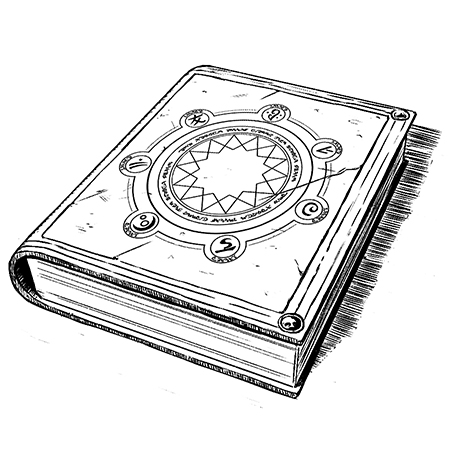
\includegraphics[width=0.7\textwidth,keepaspectratio]{mysticBook.jpg}\par
\vspace{0.4cm}
{\itshape The lore of the world contains mysteries of magic
innumerable.}\par
\vspace*{\fill}
\end{center}

\end{document}